\documentclass{article}
\usepackage[utf8]{inputenc}
\usepackage[usenames,dvipsnames]{xcolor} %monochrome option to ignore red, blue etc
\usepackage{amsmath,amssymb,graphicx, cancel, supertabular, booktabs, mathtools}
\usepackage{tikz}
\usepackage{siunitx, mhchem, comment}
%, stmaryrd}
\usepackage{bm}         % bold math fonts with \bm{}
\usepackage[font=small,labelfont=bf]{caption} % Required for specifying captions to tables and figures
\usepackage{pgfplotstable}
\usepackage{pgfplots}
\pgfplotsset{compat=1.9}
%\usepackage{lipsum}
%\frenchspacing
% bibliography
%\usepackage[backend=biber, style=numeric, bibencoding=UTF8]{biblatex}	% style=iso-numeric
%\bibliography{library.bib} 
%\journal{}
% My own styles package...
%\usepackage{customstyle}
\usepackage{wrapfig, subcaption, caption}
\usepackage{xargs}                      % Use more than one optional parameter in a new commands
\usepackage[colorinlistoftodos,prependcaption,textsize=tiny]{todonotes}
\newcommandx{\unsure}[2][1=]{\todo[linecolor=red,backgroundcolor=red!25,bordercolor=red,#1]{#2}}
\newcommandx{\change}[2][1=]{\todo[linecolor=blue,backgroundcolor=blue!25,bordercolor=blue,#1]{#2}}
\newcommandx{\info}[2][1=]{\todo[linecolor=OliveGreen,backgroundcolor=OliveGreen!25,bordercolor=OliveGreen,#1]{#2}}
\newcommandx{\improvement}[2][1=]{\todo[linecolor=Plum,backgroundcolor=Plum!25,bordercolor=Plum,#1]{#2}}
\newcommandx{\thiswillnotshow}[2][1=]{\todo[disable,#1]{#2}}

\numberwithin{equation}{section}

\usepackage[normalem]{ulem}
\usepackage[draft]{showkeys}

\definecolor{colorRed}{rgb}{0.67,0.,0.}
\definecolor{colorBlue}{rgb}{0.,0.,0.67}

\newcommand{\BR}{\color{colorRed}}
\newcommand{\ER}{\color{black}}
\newcommand{\BB}{\color{colorBlue}}
\newcommand{\EB}{\color{black}}

%\newcommand{\ara}[1]{\renewcommand{\arraystretch}{#1}}
\newcommand{\us}[1]{\underset{\textrm{s}}{#1}{}}

\def\tilde{\widetilde}
\def\cI{\mathcal{I}}
\def\F{\textrm{F}}
\def\e{\textrm{e}}
\def\Ref{\mathit{ref}}

\def\kB{k_\mathrm{B}}

\def\Ox{\mathrm{O}}
\def\oo{{\ce{O2}}}
\def\nn{{\ce{N2}}}
\def\Om{\mathrm{Om}}
\def\Oi{\mathrm{Oi}}
\def\Zr{\mathrm{Zr}}
\def\Yi{\mathrm{Y }}

\def\Mp{\mathrm{M^+}}
\def\eM{\mathrm{e^-}}


\def\MLC{M_\mathrm{C}^\mathrm{L}}
\def\MLA{M_\mathrm{A}^\mathrm{L}}
\def\nLA{n_\mathrm{A}^\mathrm{L}}
\def\nLC{n_\mathrm{C}^\mathrm{L}}
\def\nC{n_\mathrm{C}}
\def\nG{n^\mathrm{g}}
\def\nL{n_\mathrm{L}}
\def\zL{z_\mathrm{L}}
\def\zA{z_\mathrm{A}}
\def\mL{m_\mathrm{L}}
\def\vL{v_\mathrm{L}}
\def\aL{a_\mathrm{L}}

\def\DGA{\Delta G_\textrm{A}  }
\def\DGR{\Delta G_\textrm{R}  }
\def\eq{\textrm{eq}}

\def \YSZ{\textrm{YSZ}}
\def \M{\textrm{M}}

\def \yY{y^\YSZ}
\def \varphiY{\varphi^\YSZ}
\def \neM{n_\textrm{e}^\M}
\def \varphiM{\varphi^\M}

\def \yYs{{\us y}^\YSZ}
\def \neMs{\us \neM}

\def\pD{\tilde{D}}
\def\PF{P}


\def\vau{{\BB\upsilon\EB}}

\def\prms{\text{prms}}
\def\CVone{\text{CV}_1}
\def\CVtwo{\text{CV}_2}
\def\CVint{\text{CV}_\text{int}}
\def\fint{F_\text{int}}


%
%Metadata
\usepackage{hyperref}
\begin{document}
%\begin{frontmatter}
\title{CV curve interpolation}
\maketitle
%\address{Charles University, Weierstraß Institute}
%\end{frontmatter}

%\section{YSZ characterization}
%Exists in different crystalline forms, single crystal and polycrystalline shown in figures %\ref{fig:phase_d},\ref{fig:cryst}.
%For further details consult \cite{ikeda1985electrical, viazzi2008structural}.
%%\begin{figure}[h] 
%%\includegraphics[width=0.5\textwidth]{./img/phase_diagram_Scott.png}
%%\caption{}
%%\label{fig:phase_d}
%%\end{figure}
%%\begin{figure}[h] 
%%\includegraphics[width=0.7\textwidth]{./img/YSZ_crystalline_phases.png}
%%\caption{}
%%\label{fig:cryst}
%%\end{figure}
%\subsection{YSZ thermal expansion}
%\cite{hayashi2005thermal}
%Linear thermal expansion coefficient $\frac{\alpha_\textrm{V}}{3} =\alpha_\textrm{L} = \frac{1}{L}\frac{\did L}{\did T} \approx \SI{1e-6}{\per\kelvin}\text{	at }\SI{1000}{\kelvin}$.
%Grüneisen's constant $\gamma \approx 1.4$, bulk modulus $K_\textrm{T} \approx \SI{205}{\giga\pascal}@\SI{298}{\kelvin}$
%\subsection{YSZ ionic conductivity}
%The main factor driving factor is definitely temperature.
%The other factors steering the YSZ ionic conductivity are the mixing ratio $x$, crystalline structure and atmosphere.
%\subsubsection{\citeauthor{bauerle1969study}~\cite{bauerle1969study}}
%
%\subsubsection{\citeauthor{fergus2006electrolytes}~\cite{fergus2006electrolytes}, review}
%Conductivity od YSZ increases up to $8$ mole$\%$ and then decreases. The decrease at higher dopant contents might
%be due to association of point defects, which leads to reduction in defect mobility and thus conductivity.
%Size mismatch between $\ce{Zr}$ and $\ce{Y}$ leads to lower conductivity greater energy for defect association.
%
%Grain boundary conduction is said to be important.
%\begin{figure}[h]
%%\includegraphics[width=\linewidth]{./img/recherche/fergus2006_fig2.png}
%\caption{YSZ conductivities taken from~\cite{fergus2006electrolytes}, 
%apparently the value is around $\SIF{0.1}{\siemens\per\cm}$ at $\SIF{1000}{\celsius}$. }
%\end{figure}
%%
%\subsubsection{\citeauthor{chen2002influence}~\cite{chen2002influence}, granular polycrystal}
%Authors use fine-granular 8YSZ, measures EIS at temperature between $\SIF{300}{\celsius}$ and $\SIF{1000}{\celsius}$.
%Authors distinguish between intra- and intergranular conductivity, which they obtain by fitting EIS to an equivalent circuit.
%Specimen coated with a platinum paste a connected with platinum wire. Presumably air atmosphere was used.
%
%My opinion is that two different spectra are measured at high and low temperatures.
%Reported total conductivity was around $\SIF{0.1}{\siemens\per\cm}$ at
%$\SIF{1000}{\celsius}$.
%\begin{figure}[h]
%	\centering
%	%\includegraphics[width=\linewidth]{./img/recherche/chen2002_fig1.png}
%	\caption{Typical impedance spectra of YSZ at low temperature from \cite{chen2002influence}.}
%	\label{fig:chen2002}
%\end{figure}
%\subsubsection{\citeauthor{zhang2007ionic}~\cite{zhang2007ionic}}
%\begin{figure}[h]
%	\centering
%	%\includegraphics[width=\linewidth]{./img/recherche/zhang2007_fig2.png}
%	\caption{The equivalent circuit}
%	\label{fig:zhang2007}
%\end{figure}
%\subsubsection{\citeauthor{velle1991electrode}~\cite{velle1991electrode}}
%
%%\subsubsection{\citeauthor{manning1997kinetics}~\cite{manning1997kinetics}}
%Manning used $\langle 100\rangle$ single crystal 9.5YSZ and reported $\SIF{3e-2}{\siemens\per\cm}$ in $\SI{1}{\bar}$ air at $\SIF{800}{\celsius}$
%and slightly lower values in oxygen-free nitrogen.
%\vfill\eject

%%%%%%%%%%%%%%%%%%%%%%%%%%%%%%%%%%%%%%%%%%%%%%%%%%%%%%%%%%%%%%%%%%%%%%%%%%%%%%%%%%%%%




\section{Introduction}
A standard fitting process goes like:
\begin{enumerate}
\item for one fixed set of $\prms$ run FVM simulation to obtain simulated CV Curve
\item compare it with experimental CV Curve via some metric (least quares or sth.)
\item the resulting value (error) can be plotted as a point to the graph "(error / $\prms$)", e.g. Fitness Function = $f(\prms)$
\item Go To 1) until the minimum of Fitness Function is found
\end{enumerate}

If I do this procedure for more sets of parameters, lets say some point in an interval $[-0.6 , -0.1]$, we obtain some idea about the Fitness Function. But evaluating $f(\prms)$ is expensive.

\subsection{CV interpolation}
My idea is using the interpolation. Not at stage $3)$ between the points of Fitness Function itself, but on the level of $2)$. 
\\
\\
As depicted on the picture "two\_simulation.png", let us have two CV curves resulting from FVM Simulations: $\CVone$, $\CVtwo$ for $\prms = -0.6, -0.1$, respectively. I can make new CV curve as their linear interpolation in the sence

\begin{figure}
	\centering
  	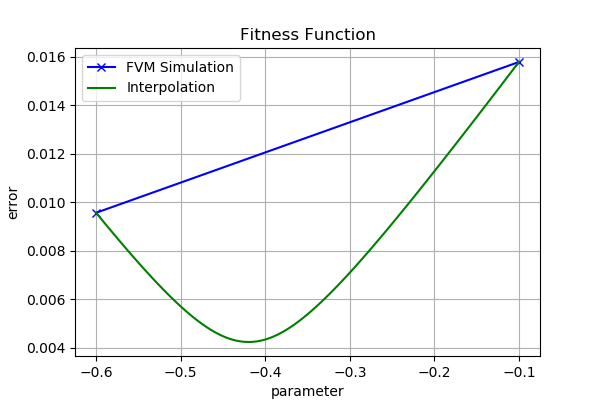
\includegraphics[scale=0.5]{./Images/FF_two.png}
	\caption{Fitness Function for $\CVone$ and $\CVtwo$.}
	\label{fig:FF_two}
\end{figure}
\begin{figure}
	\centering
  	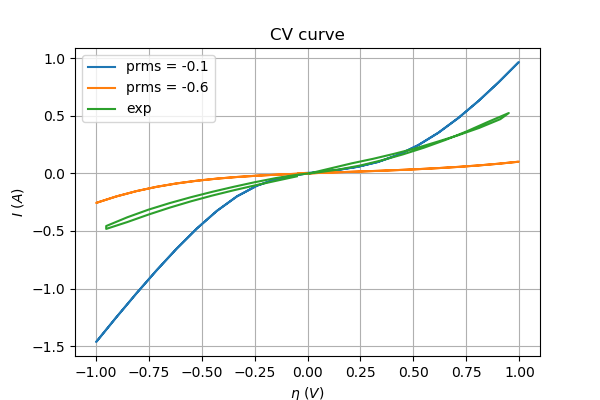
\includegraphics[scale=0.5]{./Images/CV_two.png}
	\caption{$\CVone$ and $\CVtwo$ compared to experimental CV curve.}
	\label{fig:CV_two}
\end{figure}

$$\CVint (\lambda)(U) = \CVone(U) (1 - \lambda) + \CVtwo(U) (\lambda).$$

Then for each $\lambda$ perform the comparison by metric and obtain an approximation $\fint(\lambda)$ of the true $f(\prms)$.
It turns out that we can say much more about the $f(\prms)$ than only $f(-0.6)$ and $f(-0.1)$. If the optimal $\prms^{\text{opt}}$ is in the interval, we can observe a minimum of $\fint(\lambda)$. This minimum does not have to be exatly the true minimum (see pic TODO!!!), but serves as an information where to search.

Maybe this sounds like not very useful feature, but one can divide the whole parametric space into smaller intervals, compute CV for nodes and then very cheaply interpolate in between. And then recursively explore interesting intervals more. If the true minimum is in the interval, the $\fint(\prms)$ will have extreme there (my belief, not proven yet).

When the length of parameter-space-interval is small enough, linear approximation of CV gives pretty good approximation of the true minimum.

\begin{figure}
	\centering
  	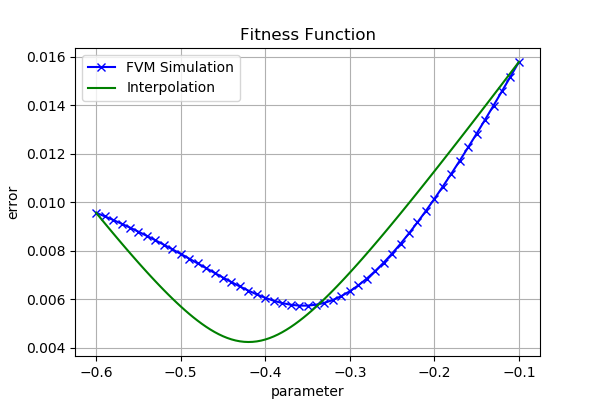
\includegraphics[scale=0.5]{./Images/FF_more.png}
	\caption{Demonstration of non-optimality of interpolated minimum.}
	\label{fig:FF_more}
\end{figure}
\begin{figure}
	\centering
  	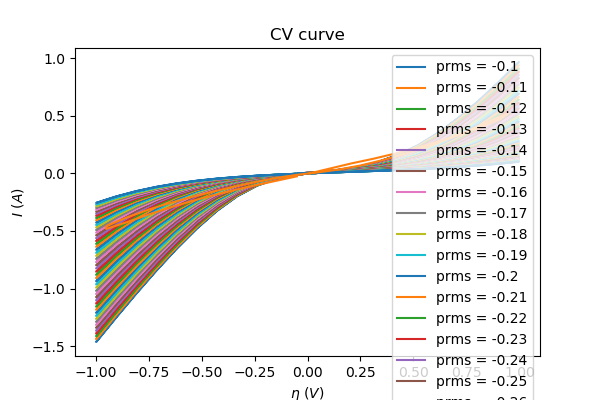
\includegraphics[scale=0.5]{./Images/CV_more.png}
	\caption{Many simulated CVs.}
	\label{fig:CV_more}
\end{figure}


\end{document}
